% options:
% thesis=B bachelor's thesis
% thesis=M master's thesis
% czech thesis in Czech language
% slovak thesis in Slovak language
% english thesis in English language
% hidelinks remove colour boxes around hyperlinks

\documentclass[thesis=B,czech]{FITthesis}[2012/06/26]

\usepackage[utf8]{inputenc} % LaTeX source encoded as UTF-8

\usepackage{graphicx} %graphics files inclusion
% \usepackage{amsmath} %advanced maths
% \usepackage{amssymb} %additional math symbols

\usepackage{dirtree} %directory tree visualisation

% % list of acronyms
% \usepackage[acronym,nonumberlist,toc,numberedsection=autolabel]{glossaries}
% \iflanguage{czech}{\renewcommand*{\acronymname}{Seznam pou{\v z}it{\' y}ch zkratek}}{}
% \makeglossaries

\newcommand{\tg}{\mathop{\mathrm{tg}}} %cesky tangens
\newcommand{\cotg}{\mathop{\mathrm{cotg}}} %cesky cotangens

% % % % % % % % % % % % % % % % % % % % % % % % % % % % % %
% ODTUD DAL VSE ZMENTE
% % % % % % % % % % % % % % % % % % % % % % % % % % % % % %

\department{Katedra \ldots softwarového inženýrství}
\title{Florbalový trenér}
\authorGN{Jakub} %(křestní) jméno (jména) autora
\authorFN{Olejník} %příjmení autora
\authorWithDegrees{Jakub Olejník} %jméno autora včetně současných akademických titulů
\supervisor{Ing. Josef Gattermayer}
\acknowledgements{Rád bych poděkoval Ing. Josefu Gattermayerovi za odborné vedení této práce a~trenérským kolektivům florbalových oddílů FbC Panthers a~AC Sparta Praha Florbal za spolupráci v~analytické části této práce.}
\abstractCS{Práce se zabývá vývojem mobilní aplikace pro tablety s~operačním systémem iOS, která si klade za cíl zjednodušit florbalovým trenérům přípravu florbalových tréninků a~cvičení. Uživatel, který aplikaci využívá, by se díky ní měl plně soustředit na obsah tréninkové jednotky nikoliv na formu, ve které ji zachytí, a~ve které ji bude následně prezentovat svým svěřencům.}
\abstractEN{The thesis deals with development of a mobile application for tablets with operating system iOS, which should simplify preparations of floorball trainings and exercises. User of this application should fully focus on the content of training unit, not the form in which it will be captured and then presented to his team.}
\placeForDeclarationOfAuthenticity{V~Praze}
\declarationOfAuthenticityOption{4} %volba Prohlášení (číslo 1-6)
\keywordsCS{florbal, trenér, trénink, iOS}
\keywordsEN{floorball, coach, training, iOS}

\begin{document}

% \newacronym{CVUT}{{\v C}VUT}{{\v C}esk{\' e} vysok{\' e} u{\v c}en{\' i} technick{\' e} v Praze}
% \newacronym{FIT}{FIT}{Fakulta informa{\v c}n{\' i}ch technologi{\' i}}

\begin{introduction}
	V~dnešním světě jsou informační technologie využívány téměř ve všech oblastech lidské činnosti, přesto se dají najít činnosti jimi nedotčené. Za takovou oblast se dají považovat mladé a~zatím neolympijské sporty, které často doplácí na podmínky amatérského prostředí. Velmi často ani špičkové oddíly nejsou schopny nabídnout svým hráčům dostatečně kvalitní zázemí. Aplikace vyvíjená v~rámci této práce by mohla tento nedostatek alespoň zmírnit.

	Toto téma jsem si zvolil na základě osobní zkušenosti a vědomí, že taková mobilní aplikace zatím neexistuje, a desktopové varianty za moc nestojí. Podobné názory jsem zaznamenal vždy když jsem na toto téma diskutoval s~jinými florbalovými trenéry. Jejich reakce na vznik takové aplikace byly vždy kladné, a proto si myslím, že navržená aplikace bude využívána a mohla by pomoci zvednout kvalitu florbalových tréninků.
\end{introduction}

\chapter{Cíl práce}
	Výsledkem práce by měl být funkční prototyp, kterým bude možné nahradit nyní využívané kreslicí tabule. Využitím tabletu se odstraní nutnost použití jiných kreslicích nástrojů, které nemusí být vždy dostupné, popř. jejich viditelnost na tabuli není dostačující. Dále elektronickou tabuli nelze umazat tak, aby na ní nebylo vysvětlované cvičení vidět, v~případě ušpinění displeje jej lze snadno očistit.

	Naopak cílem práce není aplikace určená pro libovolné kreslení. Takovou aplikaci by samozřejmě bylo možné využít i pro výše zmíněné účely, nicméně podpora symboliky, které se mezi trenéry a hráči již nyní využívá, tvoří fundamentální základ celé aplikace a~je hlavním znakem, který tuto aplikaci odlišuje od ostatních, které ji mohou svým zaměřením připomínat.

	Vytvořená aplikace nemá podporovat veškerou funkcionalitu zmíněnou v~této práci, výsledná aplikace má poskytnout dobře fungující základ, který bude možné v~budoucnu rozšiřit i o~jiné než zde zmíněné funkce.

	Zároveň je důležité navrhnout odpovídající uživatelské rozhraní, které bude dostatečně jednoduché a intuitivní. Stejně tak rozhraní nesmí odporovat zvyklostem platformy iOS, aby se uživatel v~aplikaci neztratil již po prvním spuštění.

\chapter{Analýza a návrh}

	Na začátkem práce byla provedena analýza problematiky. Byly zohledněny dobré i špatné vlastnosti již existujících aplikací nejen na iOS, ale i na OS Android a desktopových systémech. V~rámci analýzy bylo provedeno dotazníkové šetření na základě, kterého byl upraven seznam funkcí, které jsou, nebo budou implementovány. Na základě této analýzy vznikla specifikace požadavků, která bude v~této kapitole rozebrána.

\section{Analýza požadavků}

\subsection{Dotazníkové šetření}

	V rámci analytické části práce jsem se rozhodl oslovit vybraný vzorek potenciálních uživatelů aplikace. Primárním cílem tohoto šetření byla především kontrola, zda se mi podařilo zaměřit se na opravdu důležité časti aplikace. Dalším z cílů bylo získání povědomí o podobných aplikacích, které již někdo za podobným účelem použil.

	Jednotlivé body dotazníku budou rozebrány v této kapitole. Pro analýzu zmíněných podobných aplikací je připravena samostatná kapitola (\ref{sec:competition}).

\subsubsection{Cílové věkové kategorie}

	Jak je patrné z grafu \ref{graph:category}, šetření prokázalo, že cílovou skupinou budou trenéři starších kategorií (starší žáci a výše) \-- u mladších kategorií jsou priority jiné než u těch starších.

	\begin{figure}
		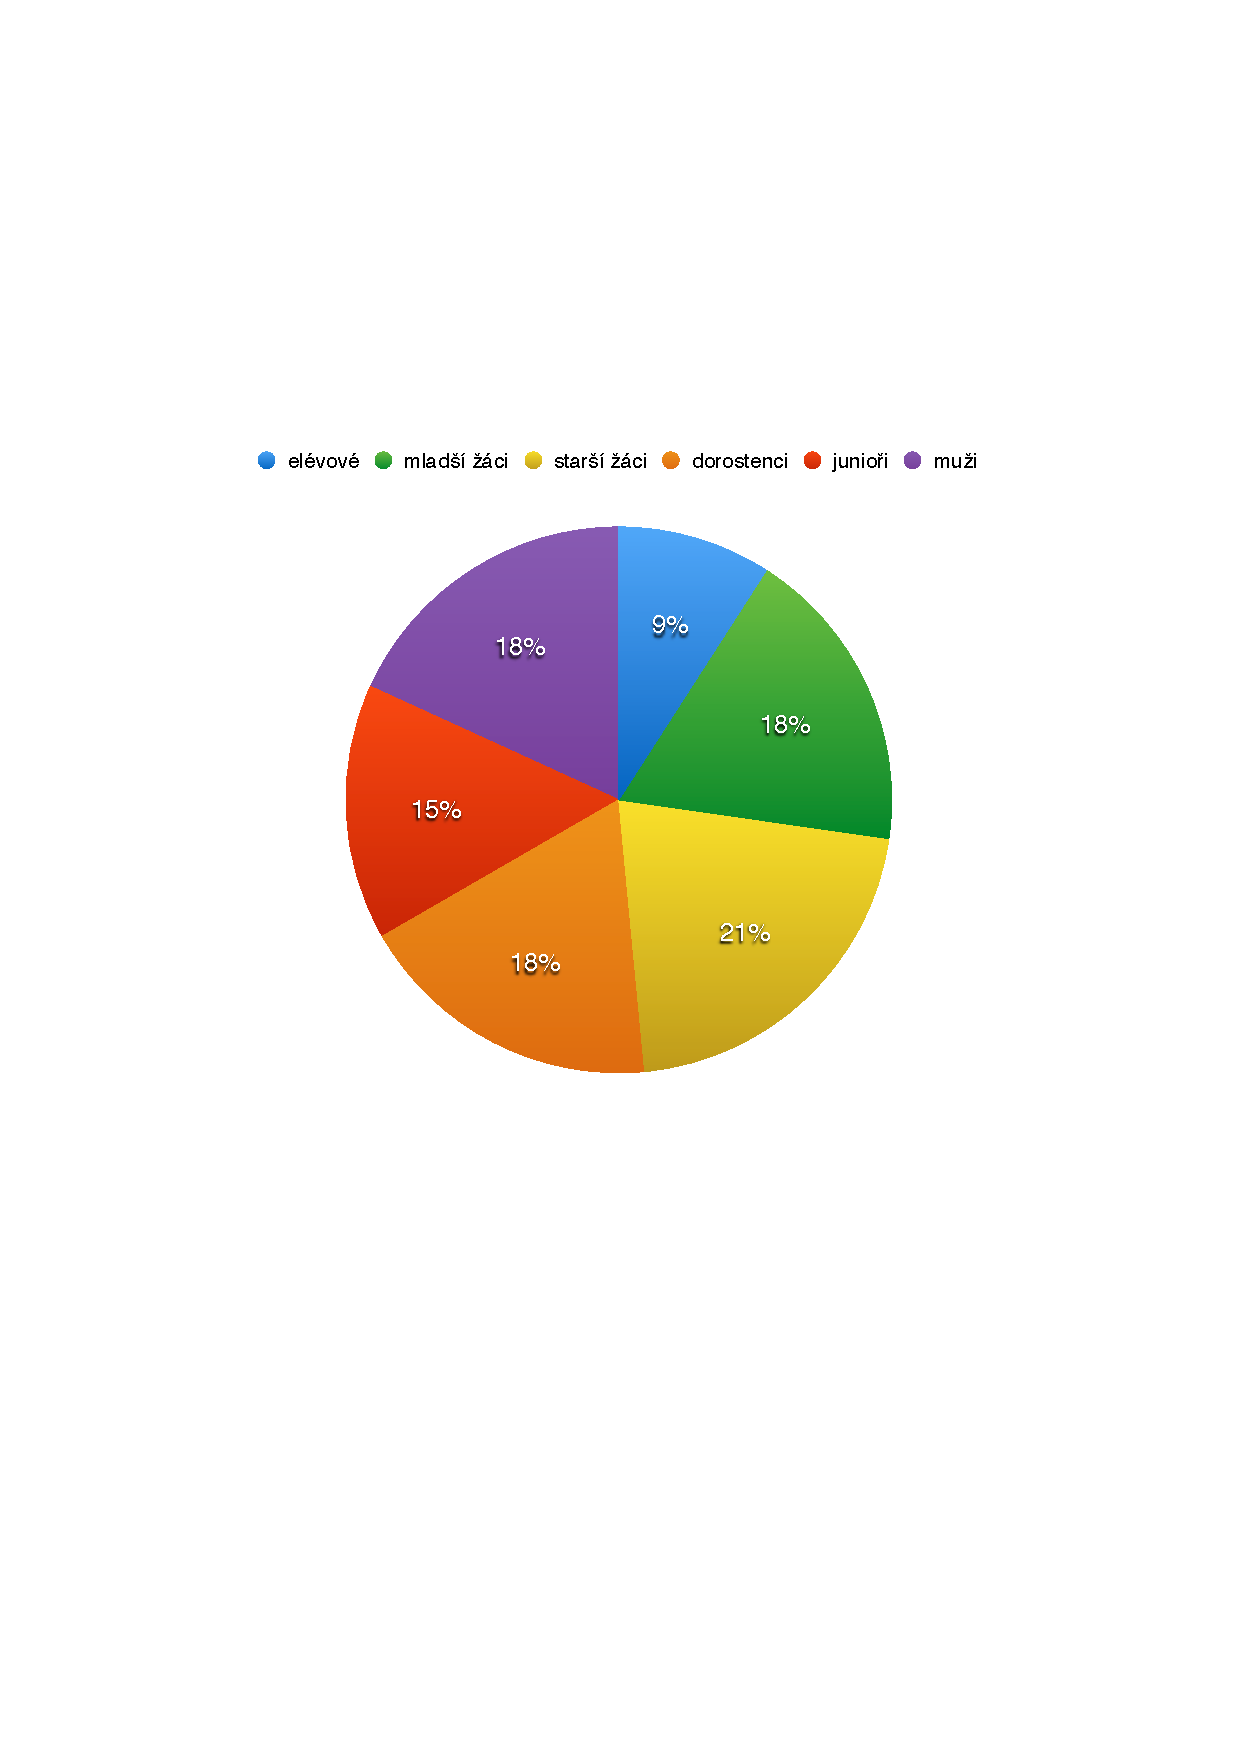
\includegraphics{img/graph_category}
		\caption{Graf trénovaných kategorií}\label{graph:category}
	\end{figure}

\subsubsection{Četnost užití kreslicí tabule}

	Dalším zjištěním (graf \ref{graph:table_usage}), které mě nepřekvapilo je fakt, že přibližně pouze pětina trenérů kreslicí tabuli nepoužívá vůbec, překvapením pro mě byla druhá část grafu \-- třetina trenérů ji využije více než pětkrát za trénink.

	\begin{figure}
		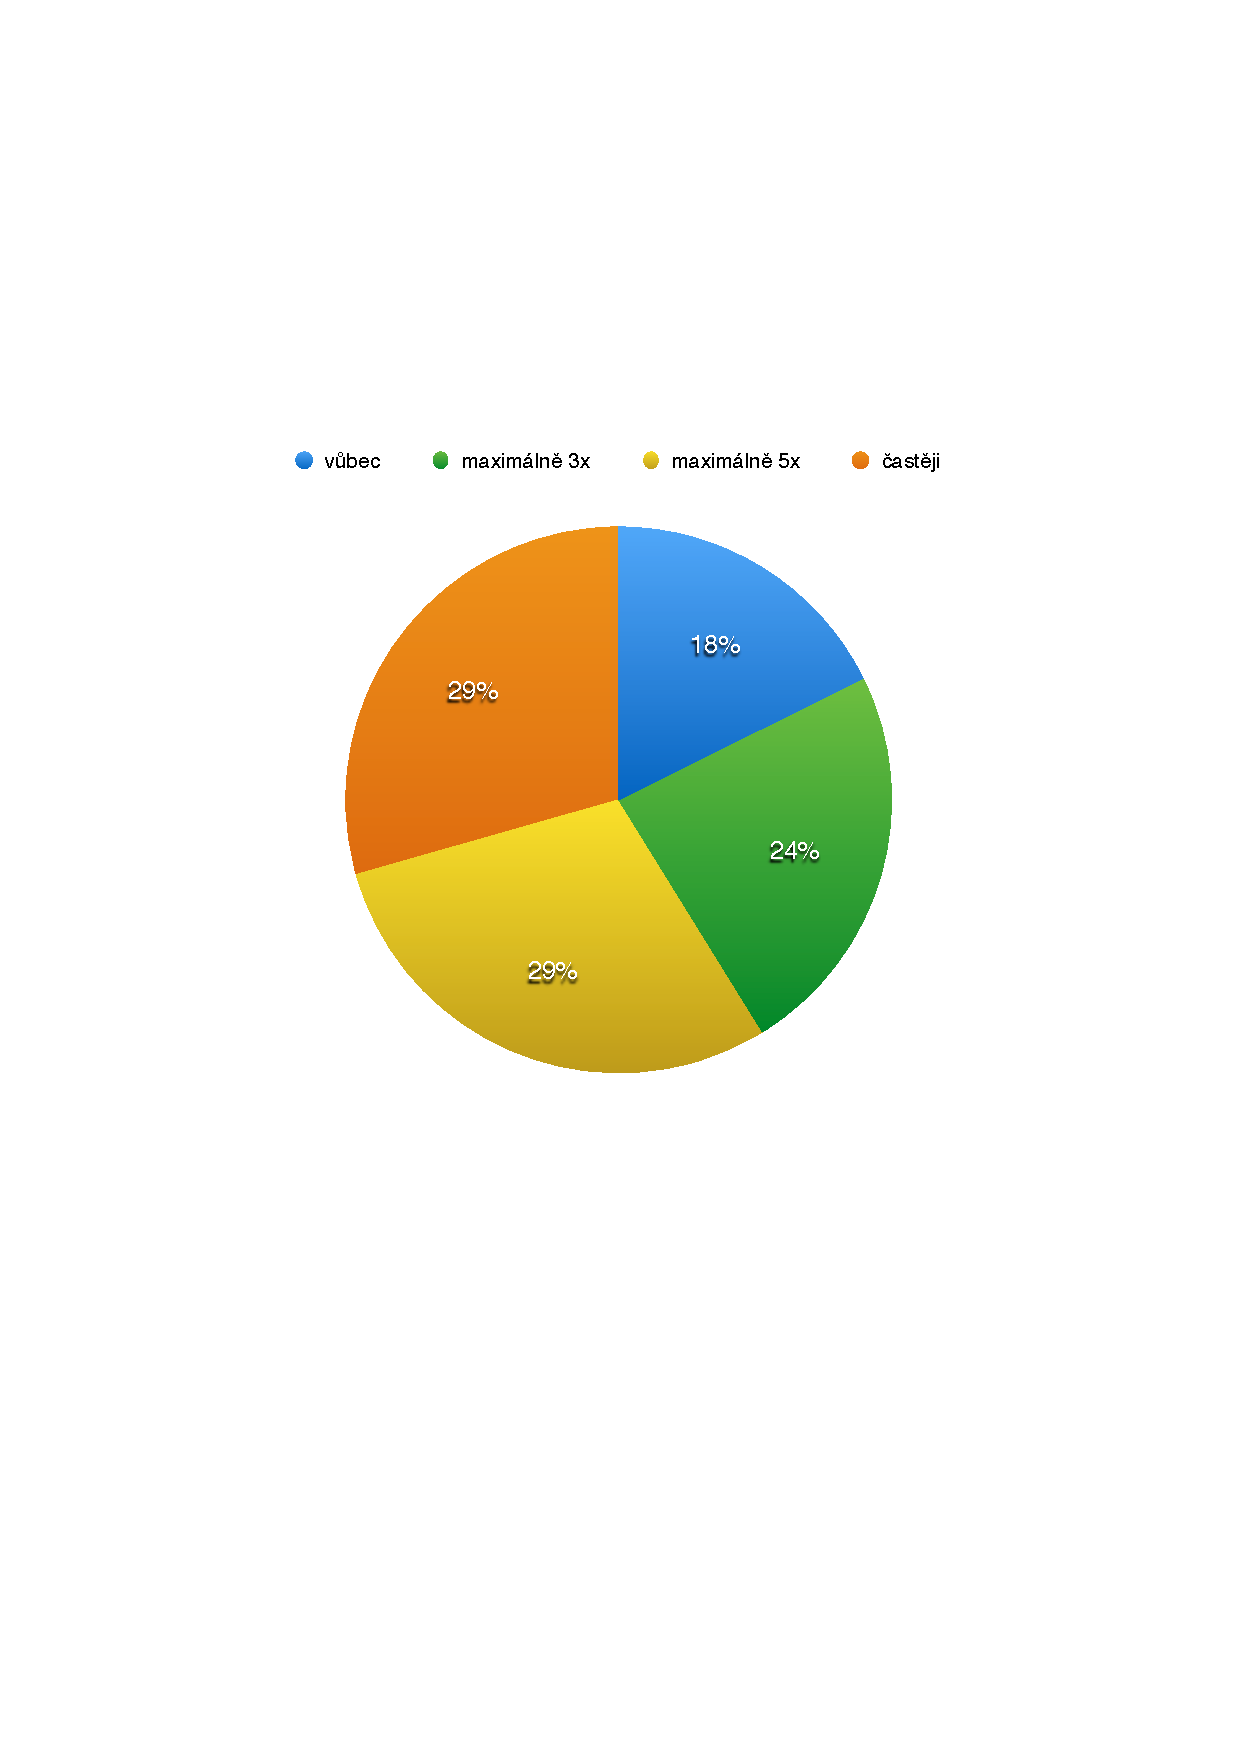
\includegraphics{img/graph_table_usage}
		\caption{Graf využívání kreslicí tabule}\label{graph:table_usage}
	\end{figure}

\subsubsection{Funkce volné kreslení, seskupování cvičení, perzistence}

	Dále se potvrdilo, že funkce volného kreslení (jako v Malování) je nepostradatelná. Toto od začátku měla být základní funkcionalita aplikace, což bylo tímto potvrzeno. Stejně zásadními funkcemi se ukázaly funkce perzistentního uložení cvičení a funkce seskupování cvičení do tréninků. Seskupováním cvičení jsem si od začátku nebyl úplně jist, ale podle tohoto výsledku jsem se rozhodl jej do aplikace zařadit.

\subsubsection{Textové poznámky}

	Naopak překvapen jsem byl tím, že textové poznámky nejsou pro trenéry tak důležité, třetina dotázaných by se bez nich obešla. Zde jsem si dovolil upřednostnit svůj hlas a do aplikace toto zařadit, protože si myslím, že poznámkový aparát může trenérovi sloužit jako upomínka, aby nezapomněl, co je důležité hráčům před cvičením zdůraznit, což vede k jejich hráčskému růstu.

\subsubsection{Automatické nakreslení cvičení}

	Zajímavou funkcionalitou, kterou bych rád v aplikaci jednou viděl je automatické postupné nakreslení cvičení. Tato funkce snižuje nároky na prezentační schopnosti trenéra tím, že jednoduchým poklepáním je schopen připravené cvičení \uv{nakreslit}. Zároveň jsou sníženy nároky na grafické nároky na trenéra, protože nemusí ve spěchu a v nepohodlné pozici cvičení kreslit. Tato funkce se líbila všem dotázaným a je na seznamu funkcí, které budou do aplikace v nejbližší době doplněny. Takto bylo rozhodnuto z důvodu její pracnosti a omezené časové dotaci na tuto práci.

	Toto byl výčet původně navrhovaných funkcí, které by měly být v aplikaci implementovány, následující funkce jsou tipy, které by dotazovaní trenéři v aplikaci ocenili.

\subsubsection{Elektronická tužka}

	Jednou z navrhovaných funkcionalit je možnost vkládání videí a jejich následný rozbor, tzv. \uv{elektronická tužka}. Tato funkce bude z aplikace kompletně vynechána. Taková funkcionalita nepatří do aplikace tohoto typu, protože aplikace se zabývá přípravou cvičení a jeho případnému vysvětlení a elektronická tužka je poněkud jiného typu.

\subsubsection{Docházka}

	Další zmíněnou funkcí byla docházka na trénink. Tato funkce nebude implementována, protože nesouvisí s přípravou tréninku. Tato funkce by mohla být zařazena do kategorie \uv{managementu} tréninku, čímž se navrhovaná aplikace nezabývá.

\subsubsection{Čas, který cvičení zabralo}

	Toto může být užitečná informace, např. ke zpětnému zhodnocení, zda bylo dobré cvičení zařadit do tréninku. Návrh vhodné implementační varianty by nejspíše vedl k rozlišení různých typů poznámek, což by mohlo být užitečné. V aktuální verzi aplikace různé typy poznámek nebudou zavedeny. To ale neznamená, že uživatel nutně o tuto informaci přijde, stále bude mít možnost si tento čas zapsat do textové poznámky.

\subsubsection{Sdílení cvičení a tréninků}

	Tato funkce již dříve byla na seznamu funkcí k prioritní implementaci. V první verzi aplikace toto podporováno nebude. Důvodem k tomuto rozhodnutí byl fakt, že k funkčnímu a pohodlnému sdílení by bylo nutné zařídit server, který by měl na starosti databázi sdílených cvičení.

	Také by se mohlo snadno stát, že místo základních funkcí, za které jsou považovány volné kreslení a užívání připravených nástrojů, by se přednostně implementovala síťová komunikace, což by mohlo vyústit k nedodržení termínu práce.

\subsubsection{Duplikace cvičení}

	Užitečnou funkcí, která se mezi odpověďmi objevila byla snadná duplikace cvičení. Motivací k takové funkcionalitě je zkušenost, že velké množství cvičení, se liší pouze v malých detailech, např. přihrávka navíc, pohyb navíc. A tak je nepraktické kreslit celé cvičení znovu, pokud je možnost cvičení zduplikovat a přihrávku tam přikreslit.



\subsection{Funkční požadavky}

\subsection{Nefunkční požadavky}

\subsection{Podporovaná zařízení}

	Operační systém iOS patří mezi velmi dynamicky se rozvíjející platformy, několikrát do roka je vydána nová verze, která obsahuje nové funkce. Toto samozřejmě může přinášet problémy se zpětnou kompatibilitou, nicméně velká většina zařízení vždy přejde na novou verzi systému téměř okamžitě, tudíž roztříštěnost tohoto systému prakticky neexistuje, což samozřejmě přináší vývojářům spoustu výhod.

	Poslední verze (verze 7) přinesla velké množství nemalých změn, především co se uživatelského rozhraní týče, a především proto jsem se rozhodl podporu starších verzí systému z aplikace vynechat.

\section{Podobné aplikace}\label{sec:competition}

\section{Návrh uživatelského rozhraní}

\chapter{Realizace}

\section{Architektura aplikace}

\section{Uživatelské rozhraní}

\chapter{Testování}

\begin{conclusion}
	%sem napište závěr Vaší práce
\end{conclusion}

\bibliographystyle{csn690}
\bibliography{mybibliographyfile}

\appendix

\chapter{Seznam použitých zkratek}
% \printglossaries
\begin{description}
	\item[GUI] Graphical user interface
	\item[XML] Extensible markup language
\end{description}


% % % % % % % % % % % % % % % % % % % % % % % % % % % %
% % Tuto kapitolu z výsledné práce ODSTRAŇTE.
% % % % % % % % % % % % % % % % % % % % % % % % % % % %
%
% \chapter{Návod k~použití této šablony}
%
% Tento dokument slouží jako základ pro napsání závěrečné práce na Fakultě informačních technologií ČVUT v~Praze.
%
% \section{Výběr základu}
%
% Vyberte si šablonu podle druhu práce (bakalářská, diplomová), jazyka (čeština, angličtina) a kódování (ASCII, \mbox{UTF-8}, \mbox{ISO-8859-2} neboli latin2 a nebo \mbox{Windows-1250}).
%
% V~české variantě naleznete šablony v~souborech pojmenovaných ve formátu práce\_kódování.tex. Typ může být:
% \begin{description}
% 	\item[BP] bakalářská práce,
% 	\item[DP] diplomová (magisterská) práce.
% \end{description}
% Kódování, ve kterém chcete psát, může být:
% \begin{description}
% 	\item[UTF-8] kódování Unicode,
% 	\item[ISO-8859-2] latin2,
% 	\item[Windows-1250] znaková sada 1250 Windows.
% \end{description}
% V~případě nejistoty ohledně kódování doporučujeme následující postup:
% \begin{enumerate}
% 	\item Otevřete šablony pro kódování UTF-8 v~editoru prostého textu, který chcete pro psaní práce použít -- pokud můžete texty s~diakritikou normálně přečíst, použijte tuto šablonu.
% 	\item V~opačném případě postupujte dále podle toho, jaký operační systém používáte:
% 	\begin{itemize}
% 		\item v~případě Windows použijte šablonu pro kódování \mbox{Windows-1250},
% 		\item jinak zkuste použít šablonu pro kódování \mbox{ISO-8859-2}.
% 	\end{itemize}
% \end{enumerate}
%
%
% V~anglické variantě jsou šablony pojmenované podle typu práce, možnosti jsou:
% \begin{description}
% 	\item[bachelors] bakalářská práce,
% 	\item[masters] diplomová (magisterská) práce.
% \end{description}
%
% \section{Použití šablony}
%
% Šablona je určena pro zpracování systémem \LaTeXe{}. Text je možné psát v~textovém editoru jako prostý text, lze však také využít specializovaný editor pro \LaTeX{}, např. Kile.
%
% Pro získání tisknutelného výstupu z~takto vytvořeného souboru použijte příkaz \verb|pdflatex|, kterému předáte cestu k~souboru jako parametr. Vhodný editor pro \LaTeX{} toto udělá za Vás. \verb|pdfcslatex| ani \verb|cslatex| \emph{nebudou} s~těmito šablonami fungovat.
%
% Více informací o~použití systému \LaTeX{} najdete např. v~\cite{wikilatex}.
%
% \subsection{Typografie}
%
% Při psaní dodržujte typografické konvence zvoleného jazyka. České \uv{uvozovky} zapisujte použitím příkazu \verb|\uv|, kterému v~parametru předáte text, jenž má být v~uvozovkách. Anglické otevírací uvozovky se v~\LaTeX{}u zadávají jako dva zpětné apostrofy, uzavírací uvozovky jako dva apostrofy. Často chybně uváděný symbol "{} (palce) nemá s~uvozovkami nic společného.
%
% Dále je třeba zabránit zalomení řádky mezi některými slovy, v~češtině např. za jednopísmennými předložkami a spojkami (vyjma \uv{a}). To docílíte vložením pružné nezalomitelné mezery -- znakem \texttt{\textasciitilde}. V~tomto případě to není třeba dělat ručně, lze použít program \verb|vlna|.
%
% Více o~typografii viz \cite{kobltypo}.
%
% \subsection{Obrázky}
%
% Pro umožnění vkládání obrázků je vhodné použít balíček \verb|graphicx|, samotné vložení se provede příkazem \verb|\includegraphics|. Takto je možné vkládat obrázky ve formátu PDF, PNG a JPEG jestliže používáte pdf\LaTeX{} nebo ve formátu EPS jestliže používáte \LaTeX{}. Doporučujeme preferovat vektorové obrázky před rastrovými (vyjma fotografií).
%
% \subsubsection{Získání vhodného formátu}
%
% Pro získání vektorových formátů PDF nebo EPS z~jiných lze použít některý z~vektorových grafických editorů. Pro převod rastrového obrázku na vektorový lze použít rasterizaci, kterou mnohé editory zvládají (např. Inkscape). Pro konverze lze použít též nástroje pro dávkové zpracování běžně dodávané s~\LaTeX{}em, např. \verb|epstopdf|.
%
% \subsubsection{Plovoucí prostředí}
%
% Příkazem \verb|\includegraphics| lze obrázky vkládat přímo, doporučujeme však použít plovoucí prostředí, konkrétně \verb|figure|. Například obrázek \ref{fig:float} byl vložen tímto způsobem. Vůbec přitom nevadí, když je obrázek umístěn jinde, než bylo původně zamýšleno -- je tomu tak hlavně kvůli dodržení typografických konvencí. Namísto vynucování konkrétní pozice obrázku doporučujeme používat odkazování z~textu (dvojice příkazů \verb|\label| a \verb|\ref|).
%
% \begin{figure}\centering
% 	
\includegraphics[width=0.5\textwidth, angle=30]{cvut-logo-bw}
% 	\caption[Příklad obrázku]{Ukázkový obrázek v~plovoucím prostředí}\label{fig:float}
% \end{figure}
%
% \subsubsection{Verze obrázků}
%
% % Gnuplot BW i barevně
% Může se hodit mít více verzí stejného obrázku, např. pro barevný či černobílý tisk a nebo pro prezentaci. S~pomocí některých nástrojů na generování grafiky je to snadné.
%
% Máte-li například graf vytvořený v programu Gnuplot, můžete jeho černobílou variantu (viz obr. \ref{fig:gnuplot-bw}) vytvořit parametrem \verb|monochrome dashed| příkazu \verb|set term|. Barevnou variantu (viz obr. \ref{fig:gnuplot-col}) vhodnou na prezentace lze vytvořit parametrem \verb|colour solid|.
%
% \begin{figure}\centering
% 	\includegraphics{gnuplot-bw}
% 	\caption{Černobílá varianta obrázku generovaného programem Gnuplot}\label{fig:gnuplot-bw}
% \end{figure}
%
% \begin{figure}\centering
% 	\includegraphics{gnuplot-col}
% 	\caption{Barevná varianta obrázku generovaného programem Gnuplot}\label{fig:gnuplot-col}
% \end{figure}
%
%
% \subsection{Tabulky}
%
% Tabulky lze zadávat různě, např. v~prostředí \verb|tabular|, avšak pro jejich vkládání platí to samé, co pro obrázky -- použijte plovoucí prostředí, v~tomto případě \verb|table|. Například tabulka \ref{tab:matematika} byla vložena tímto způsobem.
%
% \begin{table}\centering
% 	\caption[Příklad tabulky]{Zadávání matematiky}\label{tab:matematika}
% 	\begin{tabular}{|l|l|c|c|}\hline
% 		Typ		& Prostředí		& \LaTeX{}ovská zkratka	& \TeX{}ovská zkratka	\tabularnewline \hline \hline
% 		Text		& \verb|math|		& \verb|\(...\)|	& \verb|$...$|		\tabularnewline \hline
% 		Displayed	& \verb|displaymath|	& \verb|\[...\]|	& \verb|$$...$$|	\tabularnewline \hline
% 	\end{tabular}
% \end{table}
%
% % % % % % % % % % % % % % % % % % % % % % % % % % % %

\chapter{Obsah přiloženého CD}

%upravte podle skutecnosti

\begin{figure}
	\dirtree{%
		.1 readme.txt\DTcomment{stručný popis obsahu CD}.
		.1 exe\DTcomment{adresář se spustitelnou formou implementace}.
		.1 src.
		.2 impl\DTcomment{zdrojové kódy implementace}.
		.2 thesis\DTcomment{zdrojová forma práce ve formátu \LaTeX{}}.
		.1 text\DTcomment{text práce}.
		.2 thesis.pdf\DTcomment{text práce ve formátu PDF}.
		.2 thesis.ps\DTcomment{text práce ve formátu PS}.
	}
\end{figure}

\end{document}
